% MIT License

% Copyright (c) 2022 Chiyuru

% Permission is hereby granted, free of charge, to any person obtaining a copy of this software and associated documentation files (the "Software"), 
% to deal in the Software without restriction, including without limitation the rights
% to use, copy, modify, merge, publish, distribute, sublicense, and/or sell
% copies of the Software, and to permit persons to whom the Software is
% furnished to do so, subject to the following conditions:

% The above copyright notice and this permission notice shall be included in all copies or substantial portions of the Software.

% THE SOFTWARE IS PROVIDED "AS IS", WITHOUT WARRANTY OF ANY KIND, EXPRESS OR IMPLIED, INCLUDING BUT NOT LIMITED TO THE WARRANTIES OF MERCHANTABILITY,
% FITNESS FOR A PARTICULAR PURPOSE AND NONINFRINGEMENT. IN NO EVENT SHALL THE AUTHORS OR COPYRIGHT HOLDERS BE LIABLE FOR ANY CLAIM, DAMAGES OR OTHER
% LIABILITY, WHETHER IN AN ACTION OF CONTRACT, TORT OR OTHERWISE, ARISING FROM,
% OUT OF OR IN CONNECTION WITH THE SOFTWARE OR THE USE OR OTHER DEALINGS IN THE SOFTWARE.

\documentclass[UTF8]{ctexart}

\usepackage{amsmath}
\usepackage{cases}
\usepackage{cite}
\usepackage{graphicx}
\usepackage[margin=1in]{geometry}
\usepackage{float}
\geometry{a4paper}
\usepackage{fancyhdr}
\usepackage{multirow}
\pagestyle{fancy}
\fancyhf{}


\title{ICS-lab1实验报告}
\author{孔浩宇 PB20000113}
\date{\today}
\pagenumbering{arabic}

\begin{document}

\fancyhead[L]{孔浩宇}
\fancyhead[C]{ICS-lab1实验报告}
\fancyfoot[C]{\thepage}

\maketitle
\tableofcontents
\newpage

\section{实验目的}
    对于给定的数$A,\ B$,利用$LC-3$实现对$A$的后$B$位中$1$的数量的计数。

\section{实验原理}
\subsection{判断第$i$位是否为1}
    \begin{enumerate}
        \item []取$E_i = 1\times 2^{i}$,则除第$i$位为$1$外,$E_i$的其他位均为0.则
            \[
                E_i \ \& \ A[15:0] =E_i \cdot A_i .
            \]
        即对$A$的后$B$位依次与对应的$E_i$相与,若结果为0说明该位为0,否则为1.
        \end{enumerate}
\subsection{实现从第$0$位到第$B-1$位的循环判断}
    \begin{enumerate}
        \item []对于$E_i$,利用$ADD$指令,显然$E_{i+1} = E_i + E_i$,不妨设$E_i$存储在寄存器$R_k$中,则
        \[
            ADD\ R_k,\ R_k,\ R_k
            \ \Rightarrow\ 
            \mbox{此时}R_k\mbox{中的数为}2E_i=E_{i+1}.
        \]
        在$B$次循环中,结束时对$E_i$进行以上操作,可得到下一位判断所需$E_{i+1}$.
    \end{enumerate}
\subsection{实现对为1的位数的记录}
    \begin{enumerate}
        \item []使用寄存器$R_j$,初始化为0,循环判断过程中,如果该位为1 (即$E_i\ \&\ A \neq 0$),则$R_j+1$,否则跳过对$R_j$的操作.
    \end{enumerate}
\subsection{结束条件的判断}
    \begin{enumerate}
        \item []使用寄存器$R_l$,初始化为0,每次循环判断过程中,
        $R_l+1$,则当每次循环末尾,若$R_l -B<0 $,继续循环;若$R_l - B=0$,说明已经判断了后$B$位,停止循环.
    \end{enumerate}
\subsection{实现$R_j - B$}
    \begin{enumerate}
        \item []由于$LC-3$指令集中没有直接进行减法的指令,需要自己实现.首先在$R_b$中存储$B$
        \[
            R_j - B =R_j + (NOT (B) +1)
            \ \Rightarrow\ 
            \mbox{对}R_b\mbox{进行$NOT$指令后再}+1,\mbox{则}R_j + R_b = R_j -B .
        \]
    \end{enumerate}

\clearpage
\section{实验步骤}
\subsection{初始化}
\begin{enumerate}
    \item [(1)]读入$A,\ B$
    \begin{enumerate}
        \item []将存$A$的地址x3100写入地址x3012的内存,利用寄存器$R_0$来保存$A$
        \[
            1010\ 000\ 0\  0001\ 0001\quad    ;R0=M[M[x3012]]=M[x3100]=A
        \]
        \item []将存$B$的地址x3101写入地址x3013的内存,利用寄存器$R_1$来保存$B$,
        \[
            1010\ 001\ 0\ 0001\ 0001\quad    ;R1=M[M[x3013]]=M[x3101]=B
        \]
        并将$B$取反加1
        \begin{align*}
            &1001\ 001\ 001\ 000\ 000\quad    ;R1=NOT\ R1\\
            &0001\ 001\ 001\ 1\ 00001\quad    ;R1=R1+1,\mbox{now},ADD\ R1 =sub\ B
        \end{align*}
    \end{enumerate}
    \item [(2)]初始化其他变量
    \begin{align*}
        &0101\ 010\ 010\ 1\ 00000\quad    ;R2=0,\mbox{the result}\\
        &0101\ 011\ 011\ 1\ 00000\quad    ;R3=0\\
        &0001\ 100\ 011\ 1\ 00001\quad    ;R4=1\ (E_i)
    \end{align*}
\end{enumerate}

\subsection{循环}
\begin{enumerate}
    \item [(1)]循环结束判断条件
    \begin{align*}
        &0001\ 110\ 011\ 0\ 00\ 001\quad   ;R6=R3+R1=R3-B\\
        &0000\ 010\ 000\ 0\ 00\ 110\quad   ;PC+6\ \mbox{if}\ R6=0
    \end{align*}
    \item [(2)]循环过程
    \begin{align*}
        &0101\ 101\ 000\ 0\ 00\ 100\quad   ;R5=R0 \& R4\\
        &0000\ 010\ 000\ 0\ 00\ 001\quad   ;PC+1\ \mbox{if}\ R5=0\\
        &0001\ 010\ 010\ 1\ 00001\ \quad   ;R2=R2+1\\
        &0001\ 100\ 100\ 0\ 00\ 100\quad   ;R4=2*R4\\
        &0001\ 011\ 011\ 1\ 00001 \quad   ;R3=R3+1\\
        &0000\ 111\ 111\ 111\ 000 \quad   ;PC-8
    \end{align*}
\end{enumerate}

\subsection{储存结果}
    将存结果的地址x3102写入地址x3101的内存,将寄存器$R_2$的内容写入地址x3102
    \[
        1011\ 010\ 0\ 0000\ 0001\quad    ;M[M[x3011]]=M[x3102]=R2
    \]
\subsection{结束}  
    利用Trap指令结束程序
    \[
        1111\ 0000\ 0010\ 0101\quad     ;\mbox{the end}
    \]
\subsection{代码}    
    \begin{figure*}[htbp]
        \centering
        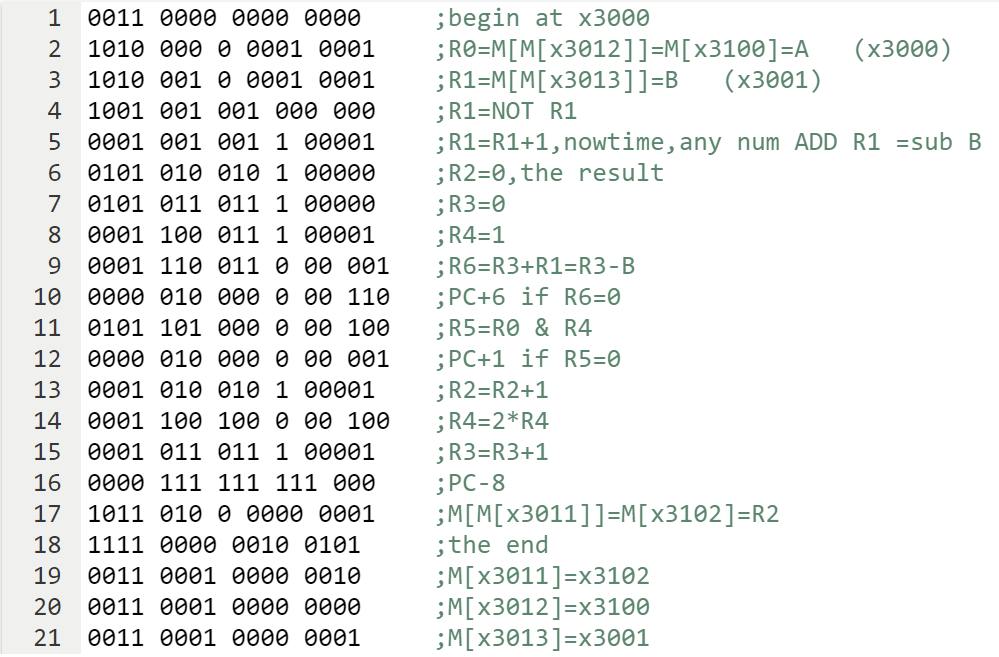
\includegraphics[scale=0.8]{code.png}
    \end{figure*}

\clearpage
\section{实验结果}
\begin{figure*}[htbp]
    \centering
    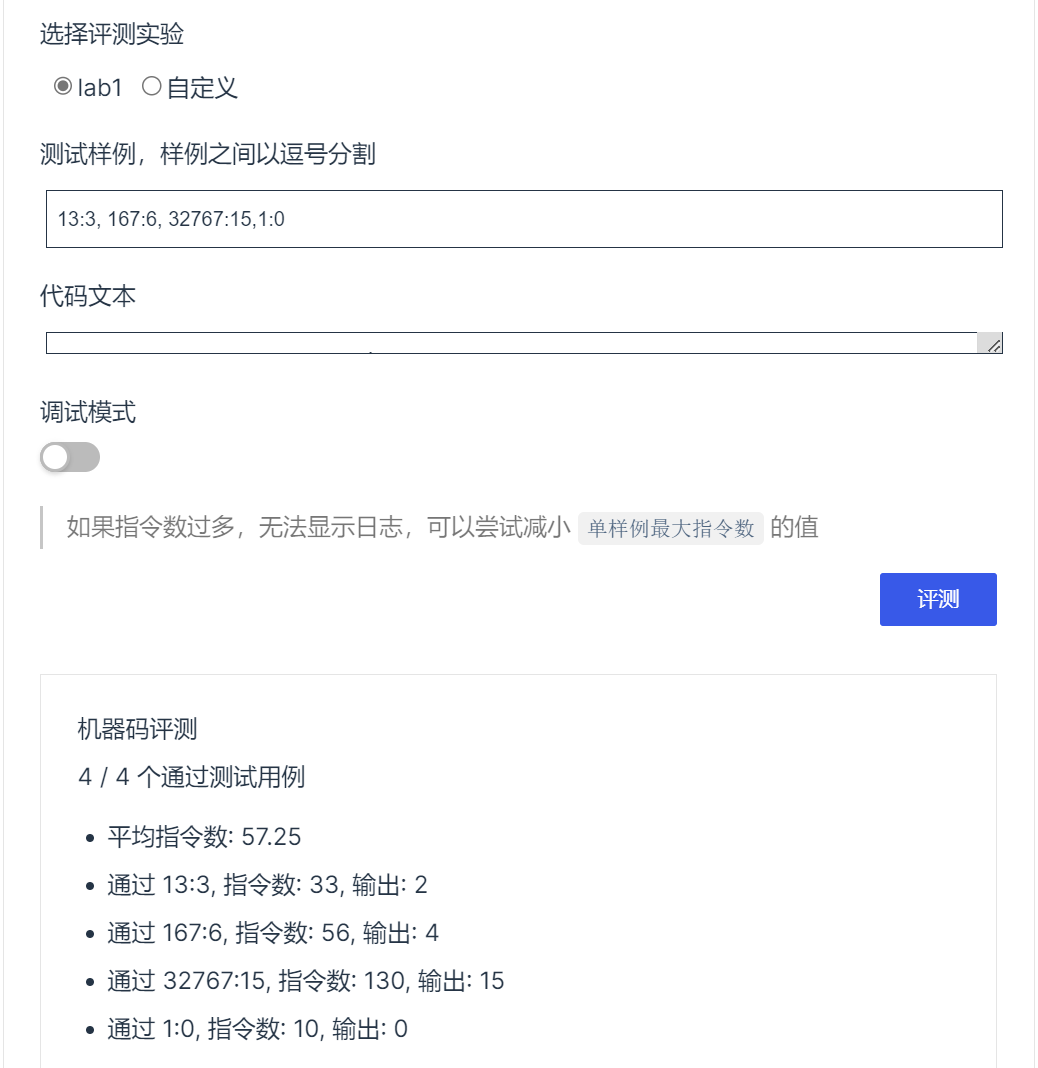
\includegraphics[scale=0.8]{result.png}
\end{figure*}

\end{document}
